\documentclass{article}
\usepackage{lipsum}
\usepackage{graphicx}
\usepackage{enumitem}
\usepackage{listings}
\usepackage{xcolor}
\usepackage{hyperref}
\usepackage{graphicx}

\title{Projektbericht: Footprint Hero - CO2-Berechnungs-App}
\author{Sebastian Koch, Philipp Zimmer}
\date{\today}

\lstdefinelanguage{Kotlin}{
  comment=[l]{//},
  commentstyle={\color{green}\ttfamily},
  emph={delegate, filter, firstOrNull, forEach, map, mapNotNull, println},
  emphstyle={\color{orange}},
  identifierstyle=\color{black},
  keywords={abstract, actual, as, as?, break, by, class, companion, continue, data, do, dynamic, else, enum, expect, false, final, for, fun, if, import, in, infix, init, inline, interface, internal, is, lateinit, noinline, null, object, open, operator, out, override, package, private, protected, public, reified, return, sealed, super, suspend, this, throw, true, try, typealias, val, var, vararg, when, where, while},
  keywordstyle={\color{blue}\bfseries},
  morecomment=[s]{/*}{*/},
  morestring=[b]",
  morestring=[s]{"""*}{*"""},
  ndkeywords={@Deprecated, @JvmField, @JvmName, @JvmOverloads, @JvmStatic, @JvmSynthetic, Array, Byte, Double, Float, Int, Integer, Iterable, Long, Runnable, Short, String, Thread, Throwable, Unit},
  ndkeywordstyle={\color{orange}\bfseries},
  sensitive=true,
  stringstyle={\color{olive}\ttfamily},
}

\lstset{
    language=Kotlin,
    basicstyle=\ttfamily,
    columns=fullflexible,
    frame=single,
    breaklines=true,
    postbreak=\mbox{\textcolor{red}{$\hookrightarrow$}\space},
}

\begin{document}

\maketitle


\section{Einleitung}
Die \textbf{Footprint Hero} App ist eine mobile Anwendung, die Benutzern hilft, bewusstere Entscheidungen zu treffen, indem sie ihre CO2-Emissionen erfassen, berechnen und verfolgen können. Footprint Hero soll den Nutzern ein generelles Bewusstsein für ihren CO2-Fußabdruck geben, indem sie über eine grafische Oberfläche einen Überblick über ihre Emissionen mit verschiedenen Fahrzeugen über verschiedene Zeiträume erhalten.

\section{Beschreibung der Funktionalität}
\begin{itemize}
	\item \textbf{Registrierung und Login}:
	
	Der Benutzer kann sich registrieren und ein Konto erstellen oder sich mit einem bestehenden Konto anmelden.
	
	\item  \textbf{Fortbewegungsmittel}:
	
	Der Benutzer kann durch Buttons von Fortbewegungsmitteln auswählen, wie er sich fortbewegt hat, einschließlich Auto, Fahrrad, Flugzeug usw.
	
	\item \textbf{Eingabe der Fortbewegungsdauer}:
	
	Der Benutzer kann die Dauer der Fortbewegung eingeben, indem er einen Radknopf dreht, um die ensprechende Dauer in Minuten-Schritten nach oben oder unten einzustellen.
	
	\item \textbf{CO2-Berechnung}:
	
	Die App berechnet automatisch den CO2-Ausstoß basierend auf der gewählten Fortbewegungsmethode und der eingegebenen Dauer.
	
	\item \textbf{Wochentagsübersicht}:
	
	Zeigt den Co2 Ausstoß tagesweise für die aktuelle Woche an, um ihm zu zeigen, ob er seinen CO2-Ausstoÿ verringert hat oder nicht.
	
	\item \textbf{Wochenübersicht}:
	
	Die App zeigt dem Benutzer eine Wochenübersicht seines CO2-Ausstoßes an und vergleicht diese mit der Vorwoche, um ihm zu zeigen, ob er seinen CO2-Aussto\ verringert hat oder nicht.
	
	\item \textbf{Benachrichtigungen}:
	
	Die App sendet dem Benutzer Benachrichtigungen, wenn er sich 30 Minutenfortbewegt hat, um ihn daran zu erinnern, seine Fortbewegungen einzugebenund um ihm eine Wochenstatistik zu senden. Diese Funktionalität wird auch zu Verfügung gestellt, wenn die App im Hintergrund läuft.
	\end{itemize}



\section{Dokumentation des Systems}
Die \textbf{Footprint Hero} App bietet eine Reihe von Funktionen, die den Benutzern dabei helfen, bewusstere Entscheidungen in Bezug auf ihre CO2-Emissionen im Verkehrssektor zu treffen. Nachfolgend werden die Funktionen im Detail erläutert:

\begin{itemize}
    \item \textbf{Verkehrsmittel- und Dauerwahl}:
    
    Benutzer können aus einer Liste von Verkehrsmitteln auswählen, darunter Auto, Bahn, Bus, Fahrrad, Taxi und Flugzeug. Diese Auswahl erfolgt über den MainScreen, der durch das \texttt{MainViewModel} gesteuert wird. Hierbei wird die ausgewählte Option des Benutzers erfasst und an das \texttt{CO2CalculationViewModel} weitergegeben. Beispielhaft dazu der Codeauszug:
    
    \begin{lstlisting}
    fun onVehicleSelected(vehicle: String) {
        selectedVehicle.value = vehicle
        co2CalculationViewModel.onVehicleSelected(vehicle)
    }
    \end{lstlisting}

    \item \textbf{CO2-Berechnung}:
    
    Die App verwendet vordefinierte Emissionswerte für verschiedene Verkehrsmittel, die im \texttt{CO2CalculationViewModel} definiert sind. Nach der Auswahl eines Verkehrsmittels und der Eingabe der Dauer berechnet die App die geschätzten CO2-Emissionen. Diese Berechnung erfolgt durch die Methode \texttt{calculateCO2} im \texttt{CO2CalculationViewModel}. Hier ist ein Beispiel, wie die CO2-Berechnung implementiert ist:
    
    \begin{lstlisting}
    fun calculateCO2() {
        val co2Emission = model.transportationCO2[model.selectedTransportation] ?: 0f
        val calculatedCo2 = (co2Emission * model.duration) / 60f
        if (!calculatedCo2.isNaN()) {
            model.co2 = calculatedCo2
        }
        Log.d("CO2CalculationModel", "Calculated CO2: $calculatedCo2")
    }
    \end{lstlisting}
    Quellen zu den Werten:
   
    
\begin{figure}
   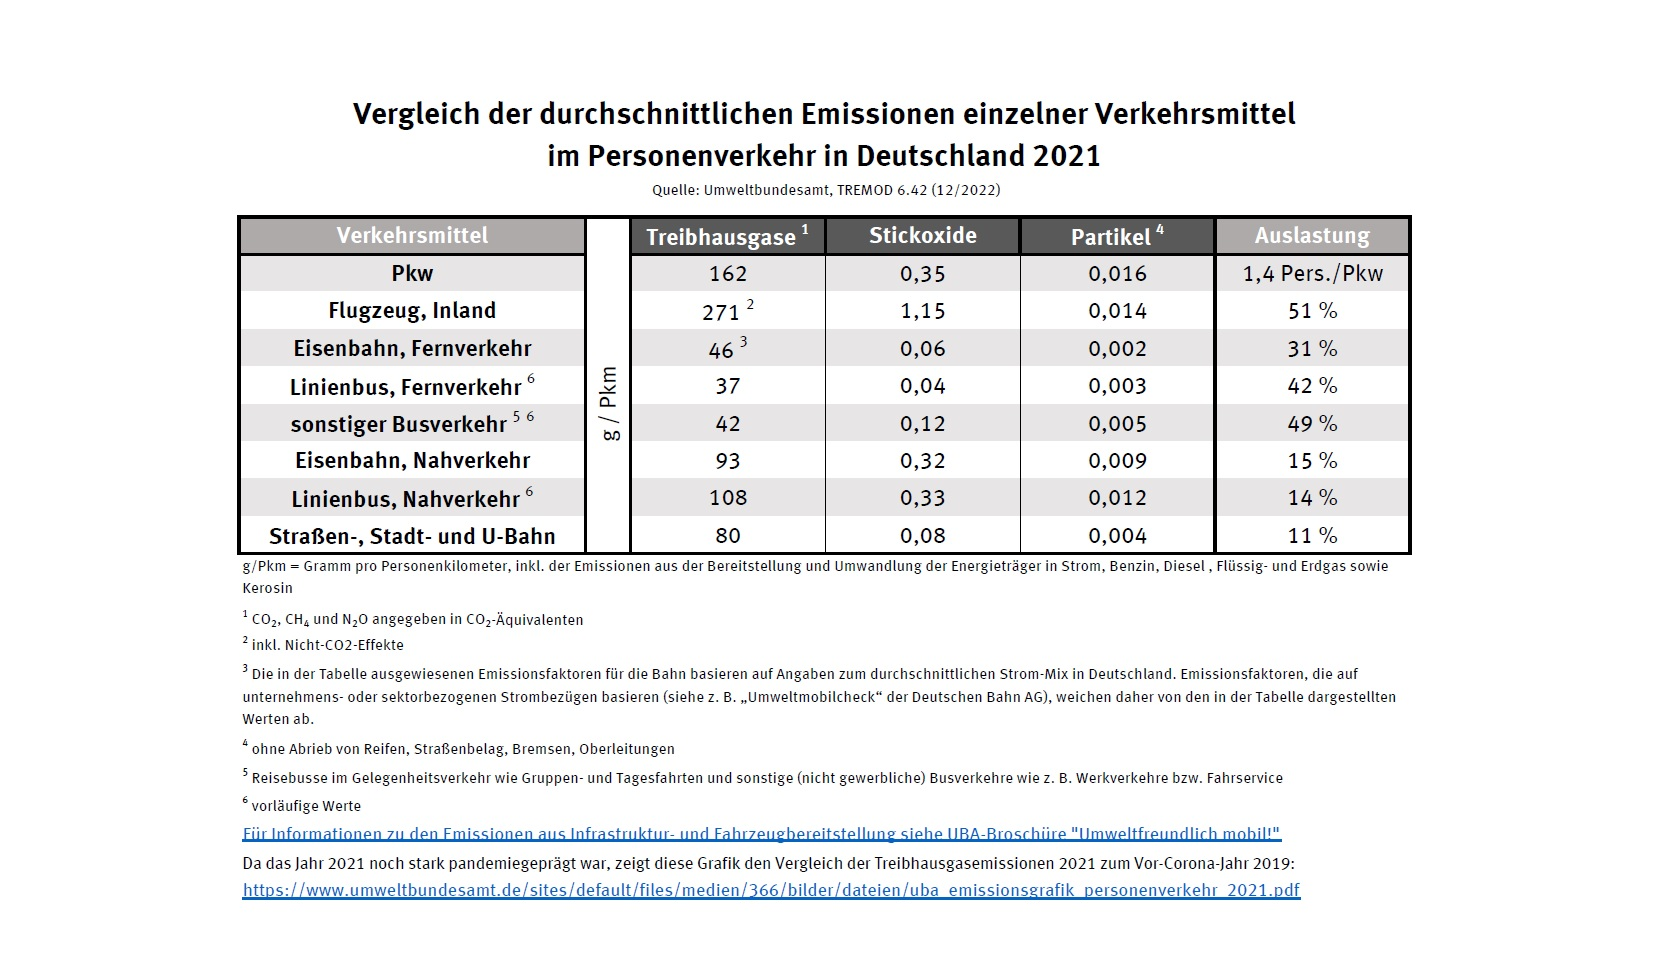
\includegraphics[width=1.00\textwidth]{uba_emissionstabelle_personenverkehr_2021_0}
   \caption{CO2 Ausstoß}
\end{figure}

    
            \item \textbf{Login}:
            
             Der LoginScreen ist der Startpunkt der App. Hier können Benutzer ihre Anmeldeinformationen eingeben, um Zugriff auf die Funktionalitäten der App zu erhalten. Der Login-Bildschirm stellt sicher, dass die persönlichen Daten und CO2-Berechnungen eines Benutzers privat und sicher bleiben.

    xxxx:
    
    \begin{lstlisting}
   \textcolor{red}{ToDo}
   
   
    \end{lstlisting}
    
    
    
        \item \textbf{Datenverfolgung}:
        
    Die berechneten CO2-Daten werden im \texttt{MainViewModel} gespeichert und verwaltet. Die Methode \texttt{merchList} aktualisiert die Liste der CO2-Daten und speichert sie in der Firebase-Datenbank. Diese Daten können dann auf dem MainScreen angezeigt werden, um den Benutzern einen Überblick über ihre CO2-Emissionen im Laufe der Zeit zu geben. Hier ist ein Beispiel für die Aktualisierung der CO2-Datenliste:
    
    \begin{lstlisting}
    private fun merchList(co2: Float) {
        // ...
        val consumptionData = ConsumptionData(
            abbreviatedDayOfWeek, co2, getCurrentCalendarWeek()
        )
        val updatedList = _co2DataList.value.co2Data.toMutableList()
        updatedList.add(consumptionData)
        _co2DataList.value = ConsumptionDataList(updatedList)
        writeCO2Data(_co2DataList.value)
        // ...
    }
    \end{lstlisting}

    \item \textbf{Bewegungserkennung}:
    
    Die App erfasst Bewegungsdaten mithilfe des Beschleunigungssensors des Geräts. Dies erfolgt durch den \texttt{MotionDetectionService}. Wenn eine Bewegungsdauer von 30 Minuten erreicht wird, zeigt die App eine Benachrichtigung an, die den Benutzer dazu auffordert, die App zu verwenden. Hier ist die Methode zur Berechnung der Bewegungsdauer:
    
    \begin{lstlisting}
    private fun calculateMotionDuration(x: Float, y: Float, z: Float): Int {
        val acceleration = sqrt(x * x + y * y + z * z)
        val motionDurationMillis = System.currentTimeMillis() - motionStartTimeMillis
        return if (acceleration > 0.1f) {
            (motionDurationMillis / (1000 * 60)).toInt()
        } else {
            0
        }
    }
    \end{lstlisting}


\item \textbf{Datenbank}:

Die \texttt{FirestoreDatabase}-Klasse behandelt die Kommunikation mit der Firebase Firestore-Datenbank. Sie bietet Methoden zum Schreiben, Lesen, Aktualisieren und Löschen von CO2-Daten.

\item \textbf{Bewegungserfassung durch den Bewegungssensor}:

Die erfassten Bewegungsdaten werden in Echtzeit abgefragt und auf eine Bewegungsdauer von 30 Minuten überprüft. Daraufhin wird eine entsprechende Notification einmalig ausgelöst.

\item \textbf{Notification}:

Die Benachrichtigung erfolgt durch die Abfrage des Bewegungssensors und wird erst nach 30 Minuten ausgelöst, wenn der Benutzer stehen bleibt. In diesem Fall startet die dreißigminütige Zählung von Neuem.  Die \texttt{NotificationHelper}-Klasse vereinfacht das Erstellen und Anzeigen von Benachrichtigungen, um Benutzer zur Verwendung der App zu motivieren.\\
Erzeugung:\\
    \begin{lstlisting}
     val notification = NotificationCompat.Builder(context, CHANNEL_ID)
            .setSmallIcon(android.R.drawable.ic_dialog_info)
            .setContentTitle("Footprint Hero calculation")
            .setContentText("You do a journy, use the Footrint Hero calulation")
            .setPriority(NotificationCompat.PRIORITY_HIGH).setContentIntent(pendingIntent)
            .setAutoCancel(true).build()
     \end{lstlisting}
     Senden:\\
     \begin{lstlisting}
      val serviceIntent = Intent(context, MyForegroundService::class.java)
                serviceIntent.putExtra("notification", notification)
                ContextCompat.startForegroundService(context, serviceIntent)
      \end{lstlisting}

\item \textbf{Observer}:

Die Absorber befinden sich im MainViewModel. Sie erfassen sämtliche Veränderungen in der Liste der CO2-Werte und informieren entsprechenden Views.
Hier die ensprechende Codestelle mit dem StateFlow:
\begin{lstlisting}
  private val _co2DataList = MutableStateFlow(ConsumptionDataList(mutableListOf()))
    val co2DataList: StateFlow<ConsumptionDataList> get() = _co2DataList
\end{lstlisting}

\item \textbf{Nebenläufigkeit}:

Die Funktionalitäten für das auslesen des Bewegungssensors und das senden der Notification als push Nachricht sind als background Operation angelegt und werden nur beim beenden der App beendet. Die Nebenläufigkeit ist umgesetzt worden durch die Verwendung der Service Klasse:
 \begin{lstlisting}
class MyForegroundService : Service() {

    companion object {
        private const val SERVICE_NOTIFICATION_ID = 1
    }

    private var notification: Notification? = null

    override fun onStartCommand(intent: Intent?, flags: Int, startId: Int): Int {
        if (intent != null) {
            notification = intent.getParcelableExtra("notification")
            if (notification != null) {
                startForeground(SERVICE_NOTIFICATION_ID, notification)
            }
        }
        return START_NOT_STICKY
    }

    override fun onBind(intent: Intent?): IBinder? {
        return null
    }

    override fun onDestroy() {
        super.onDestroy()
        stopForeground(true)
    }
}
\end{lstlisting}
\end{itemize}


\subsection{ Model-View-ViewModel (MVVM)}

Die Footprint Hero App folgt dem MVVM-Architekturmuster, das eine klare Trennung von Daten, Benutzeroberfläche und Geschäftslogik ermöglicht.
\begin{itemize}
\item \textbf{(Model)}:

Im Modellbereich werden die Datenstrukturen definiert, die zur Speicherung von Informationen verwendet werden. Die \texttt{ConsumptionData}-Klasse speichert CO2-Daten wie den Wochentag, die CO2-Emissionen und die Kalenderwoche.

\item \textbf{Sicht (View)}:

Die Benutzeroberflächenelemente und die Logik zur Anzeige von Daten werden im View-Bereich erstellt. Die Benutzerinteraktion erfolgt hier, indem sie Verkehrsmittel und Dauer auswählen. Die berechneten CO2-Daten werden angezeigt.

\item \textbf{MainScreen}:

Hier können Benutzer ihre Auswahl des Verkehrsmittels und der Dauer treffen, um die CO2-Berechnungen durchzuführen. Zusätzlich bietet der MainScreen eine Übersicht über die bisherigen CO2-Emissionen für den ausgewählten Zeitraum. Die Benutzer können auch auf die Einstellungen zugreifen, um benutzerdefinierte CO2-Emissionswerte hinzuzufügen.

%\begin{figure}[h]
    %\centering
    %\includegraphics[width=0.6\textwidth]{pfad/zum/main-screen.png}
    %\caption{MainScreen der Footprint Hero App}
    %\label{fig:main-screen}
%\end{figure}

\item \textbf{LoginScreen}:

Im LoginScreen können Benutzer ihre Anmeldeinformationen eingeben, um auf den MainScreen weitergeleitet zu werden. Der LoginScreen stellt sicher, dass die persönlichen Daten< eines Benutzers privat und sicher bleiben.

%\begin{figure}[h]
   % \centering
    %\includegraphics[width=0.4\textwidth]{pfad/zum/login-screen.png}
    %\caption{Login-Bildschirm der Footprint Hero App}
    %\label{fig:login-screen}
%\end{figure}

\item \textbf{Main(ViewModel)}:

Die \texttt{MainViewModel} Klasse stellt die Haupt ViewModel Klasse da und leitet Prozesse der User Eingabe durch die Views an entsprechende Neben ViewModel weiter und verarbeitet ensprechende Rückgaben dieser Neben Klassen.

\item \textbf{CO2CalculationViewModel}:

 Die  \texttt{CO2CalculationViewModel} ist für die Hauptfunktionalität der App verantwortlich. Sie verarbeiten die Auswahl von Verkehrsmitteln und Dauer, führen die CO2-Berechnung durch. 
 
 \item \textbf{MotionDetection}:
 
 Die \texttt{MotionDetection} Klasse verarbeitet die Sensorlogik.
 
 \item \textbf{MyForeground}:
 
 Die \texttt{MyForeground} Klasse verantwortet die Nebenläufigkeit. 
 
 \item \textbf{NotificationHelfer}:
 
 Die \texttt{NotificationHelfer} Klasse erstellt und sendet die Notification der Anwendung.
 
\end{itemize}


\section{Nicht umgesetze Ideen / Überlegungen}

    \begin{itemize}
    \item \textbf{Anpassen von co2 Werten}:
    
    Die vorhandenen CO2-Werte sollten über die GUI verändert oder gelöscht werden können. Dadurch würden die entsprechenden Daten sowohl lokal als auch in der Datenbank aktualisiert werden. Aufgrund von zeitlichen Einschränkungen konnte dies bisher jedoch noch nicht implementiert werden.
    
    \item \textbf{Gamification Elemente}:
    
    Die Integration von Gamification-Elementen entspringt einer frühen Phase der Ideenfindung und soll entsprechende Anreize zur Nutzung des Systems bieten. Es ist jedoch möglich, dass aufgrund des Umfangs dieses Konzepts bisher noch nicht in das Projekt einbezogen wurde.
    
    \item \textbf{Community Elemente}:
    
    Die Integration von Community-Elementen war zwar bereits in den frühen Planungsphasen der Ideenfindung vorhanden, wurde jedoch aufgrund des Umfangs bisher nicht in das Projekt aufgenommen. Diese Elemente sollten ebenfalls dazu dienen, die Nutzung des Systems durch die Benutzer zu fördern.
    \end{itemize}
    
    
\section{Diskussion besonderer Aspekte von Mobilität und
mobiler Software}
\begin{itemize}
\item +Verfügbarkeit des Devices, die App kann normalfall immer angewendet werden
\item +Erkennung von Bewegung des Users und möglichkeit bewegungsart zu ermitteln
\item +Notitikation in konstellation mit erkannter Bewegung
\item -viele andere Ablenkungen, durch Device und Umwelt
\item -Wenn umfangreichere Erweiterungen der App erfolgen könnte kleine Bildschirme zu herausgeforderungen werden.
\end{itemize}
    
   

\section{Reflexion über den Entwicklungsprozess}
 \begin{itemize}
    \item -Fokusierung der Appidee, entfall von community, gamification Funktionen
	\item -zeitliche Einteilung und arbeits Aufteilung war hindernis,         [gründe?], [Lektion]
	\item -\textbf{Gruppen Probleme}
	\item -Anpassung des Umfangs für die Apppfertigstellung gegen Ende 3
 	\item -Fokusierung der Entwicklung für entsprechende Meilensteine
	\item -Darstellung der App Komponenten in Bezug auf der Bildschirmgröße
	\item -Sensorik mit geschlossener App
	\item -Automatische Forbewegungsmittel erkennung
    
  \end{itemize}
  
  
\section{Teammatrix}

\begin{tabular}[h]{l|c|r}
Element & Version für Meilenstein & Finalisierung \\
\hline
Projektidee & Robin, (Sebastian) & Robin\\
\hline
MVVM & Sebastian & Philipp\\
\hline
Asynchronität & Philipp & Philipp\\
\hline
Background operations & Philipp & Philipp\\
\hline
Datenbank Anbindung & Philipp & Philipp\\
\hline
Sensor Anbindung & Philipp & Philipp\\
\hline
Notification werfen & Philipp & Philipp\\
\hline
Datenstruktur & Sebastian & Sebastian, Philipp\\
\hline
Main View & Robin & Philipp\\
\hline
Login View & Sebastian & Sebastian\\
\hline
Logik Co2 Berechnung & Robin & Philipp\\
\hline
Logik Cos Anzeige & Robin & Philipp\\
\end{tabular}

% \begin{itemize}
% \item GUI vorentwurf
 %\item MVVM
 %/item Asynchronität und background operations
 %\item Datenbank anbindung
 %\item Sensor einbinden
 %\item Notification werfen
% \item Datenstruktur
 %\item Main View
 %\item Login View
 %\item Logik für Co2 Berechnung
 %\item Logik Login
 %\item Logik Anzeige von Co2
 %\end{itemize}
    


\section{Zusammenfassung}

Die Footprint Hero App stellt eine innovative Möglichkeit dar, Benutzern bewusstere Entscheidungen im Verkehrsbereich zu ermöglichen. Mit einer klaren Architektur, die das MVVM-Muster nutzt, bietet die App eine benutzerfreundliche Benutzeroberfläche, die einfache CO2-Berechnung und -Verfolgung ermöglicht. Die Integration von Sensordaten zur Bewegungserkennung und die Verwendung von Benachrichtigungen tragen zur Steigerung der Benutzereinbindung bei. Durch die Förderung nachhaltigerer Verkehrsgewohnheiten kann die App einen positiven Beitrag zur Umwelt leisten.


\end{document}
